\documentclass{report}
\usepackage[utf8]{inputenc}

%----- Configuración del estilo del documento------%
\usepackage{epsfig,graphicx}
\usepackage[left=2.5cm,right=2.5cm,top=1.8cm,bottom=2.3cm]{geometry}
%------ Paquetes matematicos --------%
\usepackage{amsmath}
\usepackage{amssymb}
\usepackage{amsthm}
\usepackage{amsmath}
\usepackage{tabularx}
\usepackage{fancyhdr}
\usepackage{lastpage}
\usepackage{verbatim}
\usepackage[shortlabels]{enumitem}
\usepackage{venndiagram}
\usetikzlibrary{shapes.geometric}
\usepackage{cancel}
\usepackage{hyperref}
\usepackage[T1]{fontenc}
\usepackage[spanish,es-nodecimaldot,es-tabla]{babel}
\usepackage{csquotes}
\usepackage{graphicx}
\usepackage{tocloft}
\graphicspath{{./figs/}}
\usepackage{setspace}
\usepackage{xcolor}


\usepackage[backend=biber]{biblatex}
\addbibresource{resources/referencias/referencias.bib}




\begin{document}
	
	\begin{titlepage}
	\thispagestyle{empty}
	\begin{minipage}[c][0.17\textheight][c]{0.25\textwidth}
		\begin{center}
			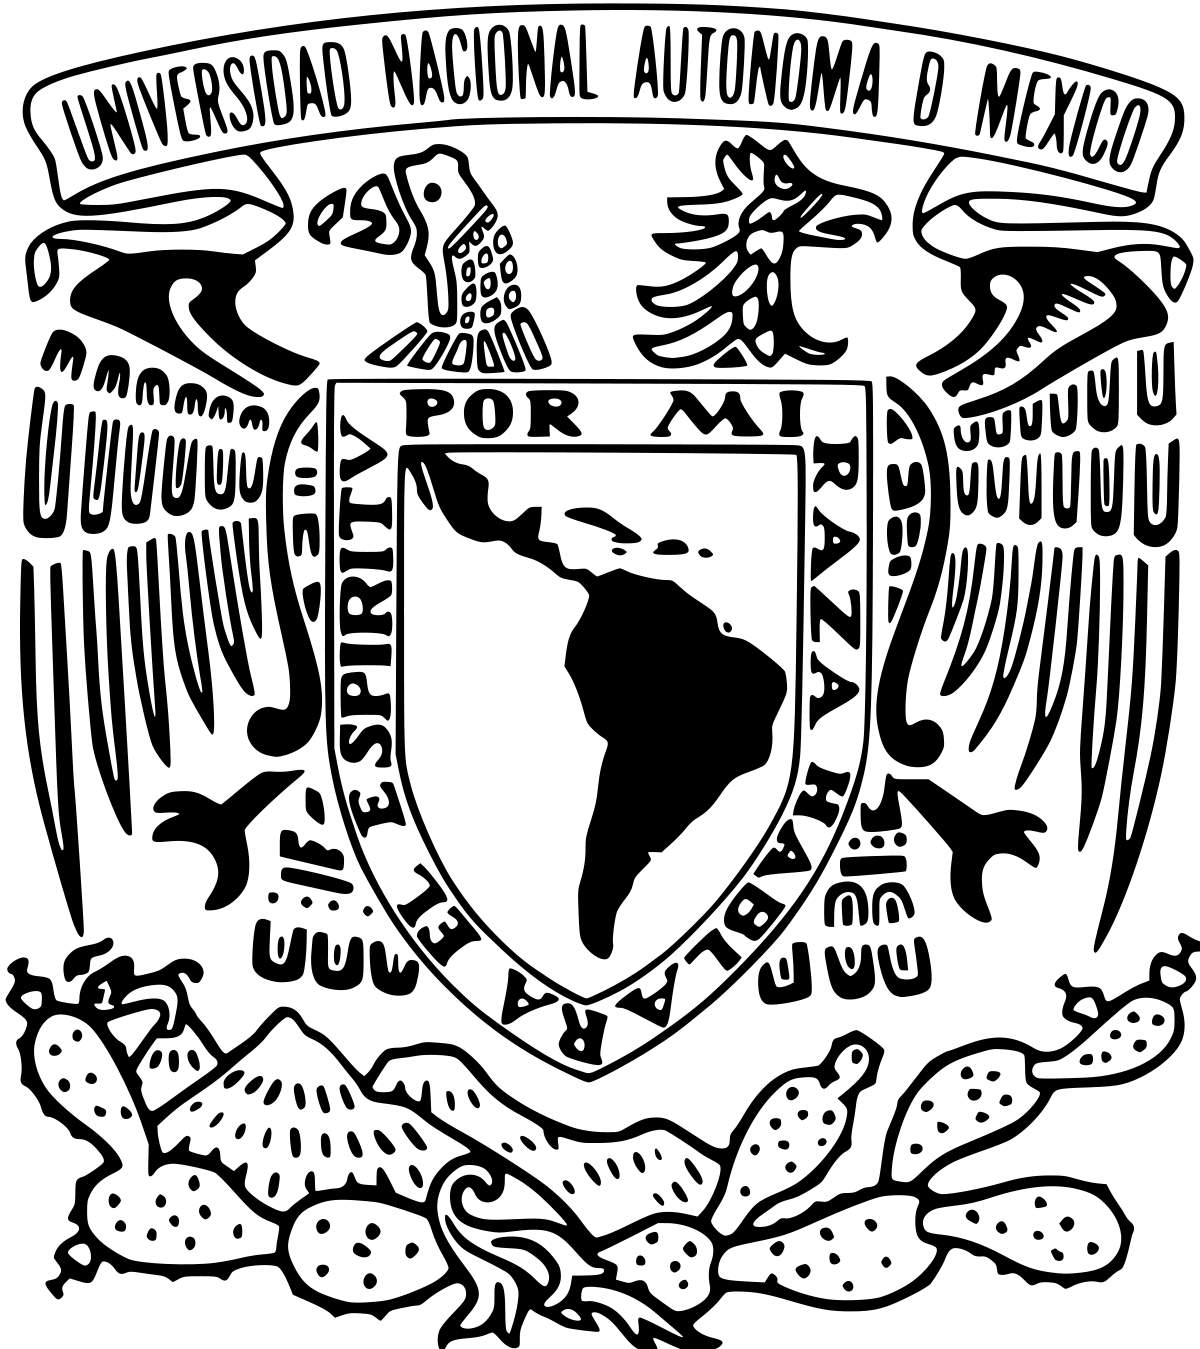
\includegraphics[width=3.5cm, height=3.5cm]{resources/Logo_UNAM.png}
		\end{center}
	\end{minipage}
	\begin{minipage}[c][0.195\textheight][t]{0.75\textwidth}
		\begin{center}
			\vspace{0.3cm}
			\textsc{\large Universidad Nacional Aut\'onoma de M\'exico}\\[0.5cm]
			\vspace{0.3cm}
			\hrule height2.5pt
			\vspace{.2cm}
			\hrule height1pt
			\vspace{.8cm}
			\textsc{Facultad de Ciencias}\\[0.5cm] %
		\end{center}
	\end{minipage}
	
	\begin{minipage}[c][0.81\textheight][t]{0.25\textwidth}
		\vspace*{5mm}
		\begin{center}
			\hskip2.0mm
			\vrule width1pt height13cm 
			\vspace{5mm}
			\hskip2pt
			\vrule width2.5pt height13cm
			\hskip2mm
			\vrule width1pt height13cm \\
			\vspace{5mm}
			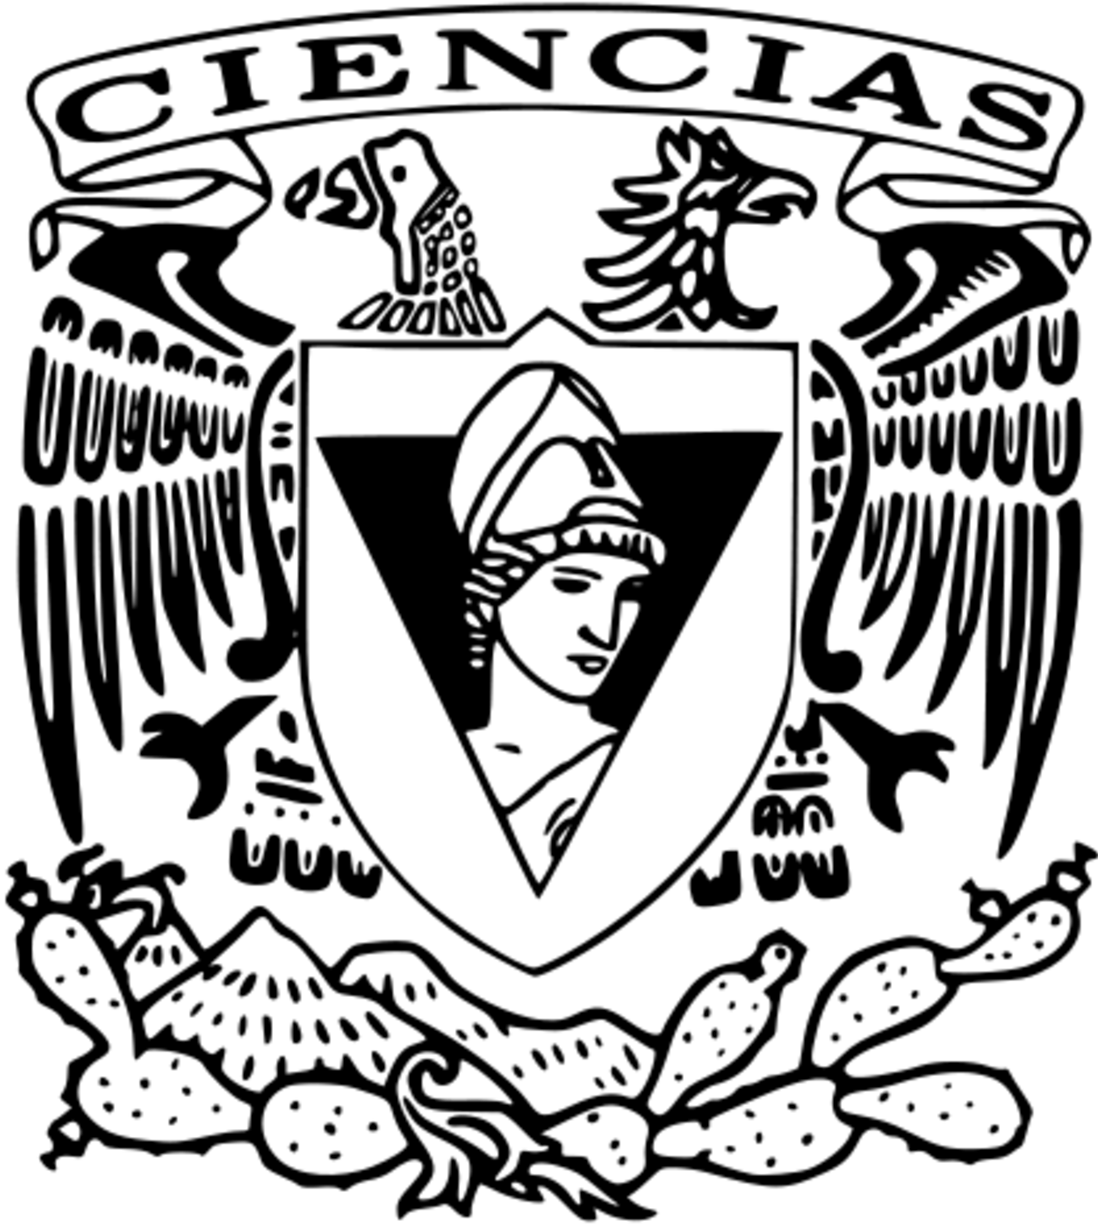
\includegraphics[height=4.0cm]{resources/Logo_FC.png}
		\end{center}
	\end{minipage}
	\begin{minipage}[c][0.81\textheight][t]{0.75\textwidth}
		\begin{center}
			\vspace{1cm}
			
			{\large\scshape Fundamentos de Bases de Datos - 7094}\\[.2in]
			
			\vspace{2cm}            
			
			\textsc{\LARGE \textbf{T}\hspace{1cm}\textbf{A}\hspace{1cm}\textbf{R}\hspace{1cm}\textbf{E}\hspace{1cm}\textbf{A}\hspace{1cm}\hspace{1cm}\textbf{4}}\\[2cm]
			\textsc{\Large{Equipo:}\normalsize \\
                \vspace{.3cm}
				\textbf{Del Monte Ortega Maryam Michelle - 320083527 \\
                \vspace{.2cm}
				\href{https://github.com/JuanSosaCiencias}{\textcolor{blue}{Sosa Romo Juan Mario - 320051926}} \\
                \vspace{.2cm}
				Castillo Hernández Antonio - 320017438 \\
                \vspace{.2cm}
                Erik Eduardo Gómez López - 320258211 \\
                \vspace{.2cm}
                Julio César Islas Espino - 320340594}}\\[0.5cm]     
			
			\textsc{{Fecha de entrega: \\ \textbf{10 de Octubre de 2024}}}\\[0.5cm]        
			
			\textsc{{Profesor: \\ \textbf{M. en I. Gerardo Avilés Rosas}}}\\[0.5cm]  
			
			\textsc{Ayudantes: \\ \textbf{Luis Enrique García Gómez \\ Kevin Jair Torres Valencia \\ Ricardo Badillo Macías \\ Rocío Aylin Huerta González
			} }
			
			
			\vspace{0.5cm}
		\end{center}
	\end{minipage}
\end{titlepage}


    \section*{\LARGE{Restauración del .backup}}

\section*{Introducción}

En esta sección, se detalla el proceso de restauración de una base de datos en un entorno de contenedores Docker utilizando PostgreSQL. Se utilizó el archivo de respaldo \texttt{transporte.backup} proporcionado por el ayudante para restaurar una base de datos de ejemplo. Este informe documenta los pasos seguidos para lograr una restauración exitosa, así como las evidencias que validan el proceso, \textit{(forma parte del punto IV de la entrega)}. \\

En escencia se siguieron los mismos pasos que se especifican en el documento de \textit{RestaurarBackupDocker.pdf} .

\section*{Pasos Realizados:} 


\subsection*{1. Verificación de Contenedores} 

Inicialmente verificamos los contenedores disponibles en Docker utilizando el comando: \\

\begin{verbatim}
    docker ps -a    
\end{verbatim}


\begin{figure}[h]
    \centering
        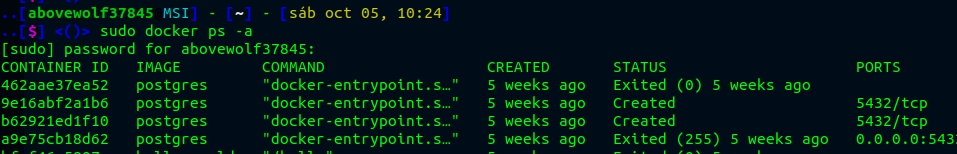
\includegraphics[width=1\textwidth]{../latex/resources/recovery/R1.png}
    \end{figure}

Despues de haber verificado los contenedores que había en el sistema, se procedió a obtener el ID de alguna de las imagenes de PostgreSQL que ya se encontraban creadas en el mismo. En este caso, se utilizó la imagen con ID \texttt{a9e75cb18d62} y procedimos a reiniciar el contenedor ya que había pasado mucho tiempo desde que se había creado. \\

\begin{figure}[h]
    \centering
        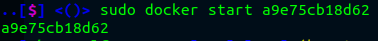
\includegraphics[width=1\textwidth]{../latex/resources/recovery/R2.png}
    \end{figure}

Checamos el estatus del contenedor con el comando \texttt{docker ps -a}. \\

\begin{figure}[h]
    \centering
        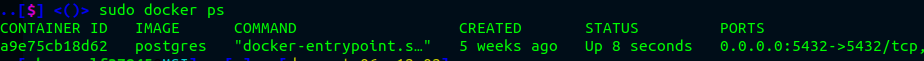
\includegraphics[width=1\textwidth]{../latex/resources/recovery/R3.png}
    \end{figure}

\subsection*{2. Conexión al Contenedor}

Una vez reiniciado el contenedor, procedimos a conectarnos a él utilizando el comando: \\

\begin{verbatim}
    sudo docker exec -it <CONTAINER_ID> psql -U postgres
\end{verbatim}

lo cual nos mete dentro de psql, una vez detro ejecutamos \textit{\l} y podemos observar lo siguiente: \\

\begin{figure}[h]
    \centering
        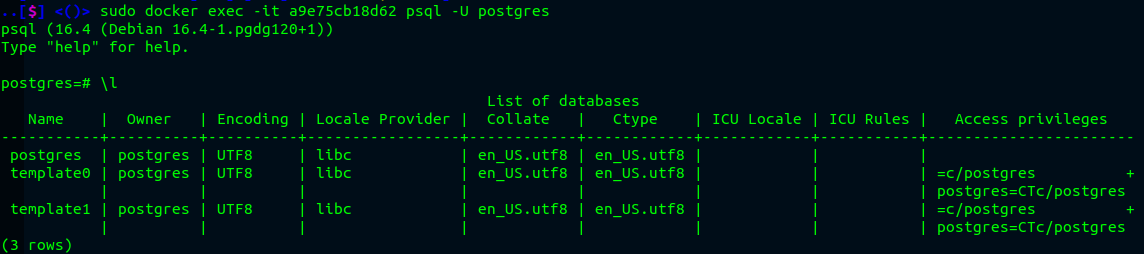
\includegraphics[width=1\textwidth]{../latex/resources/recovery/R4.png}
\end{figure}

salimos con \texttt{\textbackslash q}.

\subsection*{3. Restauración del .backup}

Como bien se menciona en el PDF, para hacer un backup necesitamos asegurarnos de que la base de datos esté vacía para evitar posibles conflictos con tablas repetidas. Entonces creamos una nueva base de datos a la cual llamaremos en esta ocasión \textit{transporte} con el ID del contenedor que hemos estado utilizando de la siguiente manera: \\

\begin{verbatim}
    sudo docker exec -it <CONTAINER_ID> createdb -U postgres ejemplo
\end{verbatim}

\begin{figure}[h!]
    \centering
        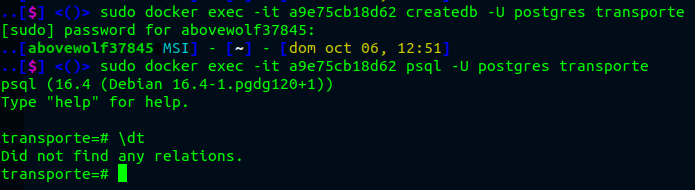
\includegraphics[width=1\textwidth]{../latex/resources/recovery/R5.png}
\end{figure}

    \newpage
	
	\begin{center}
		\section*{\LARGE{Tarea 1}}
	\end{center}

    \begin{center}
		\LARGE{\textbf{Espeficacion de reestriciones:}}\\
        \normalsize
	\end{center}
        \begin{enumerate}
            \item \section*{1. Tabla: \texttt{Pais}}
\begin{itemize}
    \item \texttt{NombrePais}: \texttt{varchar(50) NOT NULL} 
    \begin{itemize}
        \item Restricción: No puede ser nulo. Clave primaria.
    \end{itemize}
\end{itemize}

\section*{2. Tabla: \texttt{Medallero}}
\begin{itemize}
    \item \texttt{IDMedallero}: \texttt{serial PRIMARY KEY} 
    \begin{itemize}
        \item Restricción: Clave primaria generada automáticamente.
    \end{itemize}
    \item \texttt{NombrePais}: \texttt{varchar(50)} 
    \begin{itemize}
        \item Restricción: Referencia a \texttt{Pais} (clave foránea).
    \end{itemize}
\end{itemize}

\section*{3. Tabla: \texttt{Gana}}
\begin{itemize}
    \item \texttt{NombrePais}: \texttt{varchar(50) NOT NULL}
    \begin{itemize}
        \item Restricción: No puede ser nulo, clave foránea.
    \end{itemize}
    \item \texttt{TipoMedalla}: \texttt{varchar(10)}
    \begin{itemize}
        \item Restricción: Longitud máxima de 10 caracteres, clave foránea.
    \end{itemize}
    \item \texttt{IDDisciplina}: \texttt{int}
    \begin{itemize}
        \item Restricción: Clave foránea.
    \end{itemize}
    \item \textbf{PRIMARY KEY}: (\texttt{NombrePais}, \texttt{TipoMedalla}, \texttt{IDDisciplina}).
\end{itemize}

\section*{4. Tabla: \texttt{Concursa}}
\begin{itemize}
    \item \texttt{IDAtleta}: \texttt{int NOT NULL}
    \begin{itemize}
        \item Restricción: No puede ser nulo, clave foránea.
    \end{itemize}
    \item \texttt{IDEvento}: \texttt{int NOT NULL}
    \begin{itemize}
        \item Restricción: No puede ser nulo, clave foránea.
    \end{itemize}
    \item \textbf{PRIMARY KEY}: (\texttt{IDAtleta}, \texttt{IDEvento}).
\end{itemize}

\section*{5. Tabla: \texttt{TelefonoAtleta}}
\begin{itemize}
    \item \texttt{IDTelefono}: \texttt{int NOT NULL}
    \begin{itemize}
        \item Restricción: No puede ser nulo, clave primaria.
    \end{itemize}
    \item \texttt{IDAtleta}: \texttt{int}
    \begin{itemize}
        \item Restricción: Clave foránea.
    \end{itemize}
\end{itemize}

\section*{6. Tabla: \texttt{CorreoAtleta}}
\begin{itemize}
    \item \texttt{IDCorreo}: \texttt{varchar(50) NOT NULL}
    \begin{itemize}
        \item Restricción: Longitud máxima de 50 caracteres, clave primaria.
    \end{itemize}
    \item \texttt{IDAtleta}: \texttt{int}
    \begin{itemize}
        \item Restricción: Clave foránea.
    \end{itemize}
\end{itemize}

\section*{7. Tabla: \texttt{Atleta}}
\begin{itemize}
    \item \texttt{IDAtleta}: \texttt{serial PRIMARY KEY}
    \begin{itemize}
        \item Restricción: Clave primaria generada automáticamente.
    \end{itemize}
    \item \texttt{NombrePais}: \texttt{varchar(50)}
    \begin{itemize}
        \item Restricción: Clave foránea.
    \end{itemize}
    \item \texttt{IDEntrenador}: \texttt{int}
    \begin{itemize}
        \item Restricción: Clave foránea.
    \end{itemize}
    \item \texttt{Temporada}: \texttt{date default now()}
    \begin{itemize}
        \item Restricción: Fecha, valor por defecto es la fecha actual.
    \end{itemize}
    \item \texttt{Nombre}: \texttt{varchar(50) NOT NULL}
    \begin{itemize}
        \item Restricción: Longitud máxima de 50 caracteres, no puede ser nulo.
    \end{itemize}
    \item \texttt{PrimerApellido}: \texttt{varchar(50) default 'No proporcionado'}
    \begin{itemize}
        \item Restricción: Longitud máxima de 50 caracteres, valor por defecto es 'No proporcionado'.
    \end{itemize}
    \item \texttt{SegundoApellido}: \texttt{varchar(50) default 'No proporcionado'}
    \begin{itemize}
        \item Restricción: Longitud máxima de 50 caracteres, valor por defecto es 'No proporcionado'.
    \end{itemize}
    \item \texttt{FechaNacimiento}: \texttt{date NOT NULL}
    \begin{itemize}
        \item Restricción: No puede ser nulo.
    \end{itemize}
    \item \texttt{Nacionalidad}: \texttt{varchar(50) default 'No proporcionado'}
    \begin{itemize}
        \item Restricción: Longitud máxima de 50 caracteres, valor por defecto es 'No proporcionado'.
    \end{itemize}
    \item \texttt{Genero}: \texttt{char(1) default 0}
    \begin{itemize}
        \item Restricción: Un solo carácter, valor por defecto es 0.
    \end{itemize}
\end{itemize}

\section*{8. Tabla: \texttt{Participa}}
\begin{itemize}
    \item \texttt{IDAtleta}: \texttt{int NOT NULL}
    \begin{itemize}
        \item Restricción: No puede ser nulo, clave foránea.
    \end{itemize}
    \item \texttt{IDDisciplina}: \texttt{int NOT NULL}
    \begin{itemize}
        \item Restricción: No puede ser nulo, clave foránea.
    \end{itemize}
    \item \textbf{PRIMARY KEY}: (\texttt{IDAtleta}, \texttt{IDDisciplina}).
\end{itemize}

\section*{9. Tabla: \texttt{Medalla}}
\begin{itemize}
    \item \texttt{TipoMedalla}: \texttt{varchar(10) NOT NULL}
    \begin{itemize}
        \item Restricción: Longitud máxima de 10 caracteres, no puede ser nulo.
    \end{itemize}
    \item \texttt{IDDisciplina}: \texttt{int NOT NULL}
    \begin{itemize}
        \item Restricción: No puede ser nulo, clave foránea.
    \end{itemize}
    \item \textbf{PRIMARY KEY}: (\texttt{TipoMedalla}, \texttt{IDDisciplina}).
\end{itemize}

\section*{10. Tabla: \texttt{Evento}}
\begin{itemize}
    \item \texttt{IDEvento}: \texttt{serial PRIMARY KEY}
    \begin{itemize}
        \item Restricción: Clave primaria generada automáticamente.
    \end{itemize}
    \item \texttt{NombreLocalidad}: \texttt{varchar(50)}
    \begin{itemize}
        \item Restricción: Clave foránea.
    \end{itemize}
    \item \texttt{IDDisciplina}: \texttt{int}
    \begin{itemize}
        \item Restricción: Clave foránea.
    \end{itemize}
    \item \texttt{DuracionMax}: \texttt{int NOT NULL}
    \begin{itemize}
        \item Restricción: No puede ser nulo.
    \end{itemize}
    \item \texttt{Precio}: \texttt{int NOT NULL}
    \begin{itemize}
        \item Restricción: No puede ser nulo.
    \end{itemize}
    \item \texttt{FechaEvento}: \texttt{date NOT NULL}
    \begin{itemize}
        \item Restricción: No puede ser nulo.
    \end{itemize}
    \item \texttt{Fase}: \texttt{int default 0}
    \begin{itemize}
        \item Restricción: Valor entero, valor por defecto es 0.
    \end{itemize}
\end{itemize}

\section*{11. Tabla: \texttt{TelefonoEntrenador}}
\begin{itemize}
    \item \texttt{IDTelefono}: \texttt{int NOT NULL}
    \begin{itemize}
        \item Restricción: No puede ser nulo, clave primaria.
    \end{itemize}
    \item \texttt{IDEntrenador}: \texttt{int}
    \begin{itemize}
        \item Restricción: Clave foránea.
    \end{itemize}
\end{itemize}

\section*{12. Tabla: \texttt{Disciplina}}
\begin{itemize}
    \item \texttt{IDDisciplina}: \texttt{serial PRIMARY KEY}
    \begin{itemize}
        \item Restricción: Clave primaria generada automáticamente.
    \end{itemize}
    \item \texttt{NombreDisciplina}: \texttt{varchar(50) NOT NULL}
    \begin{itemize}
        \item Restricción: Longitud máxima de 50 caracteres, no puede ser nulo.
    \end{itemize}
    \item \texttt{Categoria}: \texttt{varchar(50) NOT NULL}
    \begin{itemize}
        \item Restricción: Longitud máxima de 50 caracteres, no puede ser nulo.
    \end{itemize}
\end{itemize}

\section*{13. Tabla: \texttt{Localidad}}
\begin{itemize}
    \item \texttt{NombreLocalidad}: \texttt{varchar(50) NOT NULL}
    \begin{itemize}
        \item Restricción: Longitud máxima de 50 caracteres, clave primaria.
    \end{itemize}
    \item \texttt{IDDisciplina}: \texttt{int NOT NULL}
    \begin{itemize}
        \item Restricción: Clave foránea, no puede ser nulo.
    \end{itemize}
    \item \texttt{Calle}: \texttt{varchar(50) NOT NULL}
    \begin{itemize}
        \item Restricción: Longitud máxima de 50 caracteres, no puede ser nulo.
    \end{itemize}
    \item \texttt{Numero}: \texttt{int NOT NULL}
    \begin{itemize}
        \item Restricción: No puede ser nulo.
    \end{itemize}
    \item \texttt{Ciudad}: \texttt{varchar(50) NOT NULL}
    \begin{itemize}
        \item Restricción: Longitud máxima de 50 caracteres, no puede ser nulo.
    \end{itemize}
    \item \texttt{Pais}: \texttt{varchar(50) NOT NULL}
    \begin{itemize}
        \item Restricción: Longitud máxima de 50 caracteres, no puede ser nulo.
    \end{itemize}
    \item \texttt{Aforo}: \texttt{int NOT NULL}
    \begin{itemize}
        \item Restricción: No puede ser nulo.
    \end{itemize}
    \item \texttt{Tipo}: \texttt{int NOT NULL}
    \begin{itemize}
        \item Restricción: No puede ser nulo.
    \end{itemize}
\end{itemize}

\section*{14. Tabla: \texttt{CompraEntrada}}
\begin{itemize}
    \item \texttt{IDCliente}: \texttt{int NOT NULL}
    \begin{itemize}
        \item Restricción: No puede ser nulo, clave foránea.
    \end{itemize}
    \item \texttt{IDEvento}: \texttt{int NOT NULL}
    \begin{itemize}
        \item Restricción: No puede ser nulo, clave foránea.
    \end{itemize}
    \item \textbf{PRIMARY KEY}: (\texttt{IDCliente}, \texttt{IDEvento}).
\end{itemize}

\section*{15. Tabla: \texttt{Cliente}}
\begin{itemize}
    \item \texttt{IDCliente}: \texttt{serial PRIMARY KEY}
    \begin{itemize}
        \item Restricción: Clave primaria generada automáticamente.
    \end{itemize}
    \item \texttt{Nombre}: \texttt{varchar(50) NOT NULL}
    \begin{itemize}
        \item Restricción: Longitud máxima de 50 caracteres, no puede ser nulo.
    \end{itemize}
    \item \texttt{Correo}: \texttt{varchar(50) NOT NULL}
    \begin{itemize}
        \item Restricción: Longitud máxima de 50 caracteres, no puede ser nulo.
    \end{itemize}
    \item \texttt{Telefono}: \texttt{varchar(10)}
    \begin{itemize}
        \item Restricción: Longitud máxima de 10 caracteres.
    \end{itemize}
\end{itemize}

\section*{16. Tabla: \texttt{CorreoEntrenador}}
\begin{itemize}
    \item \texttt{IDCorreo}: \texttt{varchar(50) NOT NULL}
    \begin{itemize}
        \item Restricción: Longitud máxima de 50 caracteres, no puede ser nulo, clave primaria.
    \end{itemize}
    \item \texttt{IDEntrenador}: \texttt{int}
    \begin{itemize}
        \item Restricción: Clave foránea.
    \end{itemize}
\end{itemize}

\section*{17. Tabla: \texttt{Entrenador}}
\begin{itemize}
    \item \texttt{IDEntrenador}: \texttt{serial PRIMARY KEY}
    \begin{itemize}
        \item Restricción: Clave primaria generada automáticamente.
    \end{itemize}
    \item \texttt{IDDisciplina}: \texttt{int}
    \begin{itemize}
        \item Restricción: Clave foránea.
    \end{itemize}
    \item \texttt{Nombre}: \texttt{varchar(50) NOT NULL}
    \begin{itemize}
        \item Restricción: Longitud máxima de 50 caracteres, no puede ser nulo.
    \end{itemize}
    \item \texttt{PrimerApellido}: \texttt{varchar(50) default 'No proporcionado'}
    \begin{itemize}
        \item Restricción: Longitud máxima de 50 caracteres, valor por defecto es 'No proporcionado'.
    \end{itemize}
    \item \texttt{SegundoApellido}: \texttt{varchar(50) default 'No proporcionado'}
    \begin{itemize}
        \item Restricción: Longitud máxima de 50 caracteres, valor por defecto es 'No proporcionado'.
    \end{itemize}
    \item \texttt{FechaNacimiento}: \texttt{date NOT NULL}
    \begin{itemize}
        \item Restricción: No puede ser nulo.
    \end{itemize}
    \item \texttt{Nacionalidad}: \texttt{varchar(50) default 'No proporcionado'}
    \begin{itemize}
        \item Restricción: Longitud máxima de 50 caracteres, valor por defecto es 'No proporcionado'.
    \end{itemize}
    \item \texttt{Genero}: \texttt{char(1) default 0}
    \begin{itemize}
        \item Restricción: Un solo carácter, valor por defecto es 0.
    \end{itemize}
\end{itemize}

\section*{18. Tabla: \texttt{TelefonoArbitro}}
\begin{itemize}
    \item \texttt{IDTelefono}: \texttt{int NOT NULL}
    \begin{itemize}
        \item Restricción: No puede ser nulo, clave primaria.
    \end{itemize}
    \item \texttt{IDArbitro}: \texttt{int}
    \begin{itemize}
        \item Restricción: Clave foránea.
    \end{itemize}
\end{itemize}

\section*{19. Tabla: \texttt{Patrocina}}
\begin{itemize}
    \item \texttt{NombrePatrocinador}: \texttt{varchar(50) NOT NULL}
    \begin{itemize}
        \item Restricción: No puede ser nulo, clave foránea.
    \end{itemize}
    \item \texttt{IDDisciplina}: \texttt{int NOT NULL}
    \begin{itemize}
        \item Restricción: No puede ser nulo, clave foránea.
    \end{itemize}
    \item \textbf{PRIMARY KEY}: (\texttt{NombrePatrocinador}, \texttt{IDDisciplina}).
\end{itemize}

\section*{20. Tabla: \texttt{Arbitro}}
\begin{itemize}
    \item \texttt{IDArbitro}: \texttt{serial PRIMARY KEY}
    \begin{itemize}
        \item Restricción: Clave primaria generada automáticamente.
    \end{itemize}
    \item \texttt{IDDisciplina}: \texttt{int}
    \begin{itemize}
        \item Restricción: Clave foránea.
    \end{itemize}
    \item \texttt{Nombre}: \texttt{varchar(50) NOT NULL}
    \begin{itemize}
        \item Restricción: Longitud máxima de 50 caracteres, no puede ser nulo.
    \end{itemize}
    \item \texttt{PrimerApellido}: \texttt{varchar(50) default 'No proporcionado'}
    \begin{itemize}
        \item Restricción: Longitud máxima de 50 caracteres, valor por defecto es 'No proporcionado'.
    \end{itemize}
    \item \texttt{SegundoApellido}: \texttt{varchar(50) default 'No proporcionado'}
    \begin{itemize}
        \item Restricción: Longitud máxima de 50 caracteres, valor por defecto es 'No proporcionado'.
    \end{itemize}
    \item \texttt{FechaNacimiento}: \texttt{date NOT NULL}
    \begin{itemize}
        \item Restricción: No puede ser nulo.
    \end{itemize}
    \item \texttt{Nacionalidad}: \texttt{varchar(50) default 'No proporcionado'}
    \begin{itemize}
        \item Restricción: Longitud máxima de 50 caracteres, valor por defecto es 'No proporcionado'.
    \end{itemize}
    \item \texttt{Genero}: \texttt{char(1) default 0}
    \begin{itemize}
        \item Restricción: Un solo carácter, valor por defecto es 0.
    \end{itemize}
\end{itemize}

\section*{21. Tabla: \texttt{CorreoArbitro}}
\begin{itemize}
    \item \texttt{IDCorreo}: \texttt{varchar(50) NOT NULL}
    \begin{itemize}
        \item Restricción: Longitud máxima de 50 caracteres, clave primaria.
    \end{itemize}
    \item \texttt{IDArbitro}: \texttt{int}
    \begin{itemize}
        \item Restricción: Clave foránea.
    \end{itemize}
\end{itemize}

\section*{22. Tabla: \texttt{Patrocinador}}
\begin{itemize}
    \item \texttt{NombrePatrocinador}: \texttt{varchar(50) NOT NULL}
    \begin{itemize}
        \item Restricción: Longitud máxima de 50 caracteres, clave primaria.
    \end{itemize}
\end{itemize}


\section{Modelo Entidad Relación de la Práctica 4:}
\begin{figure}[H]
    \centering
    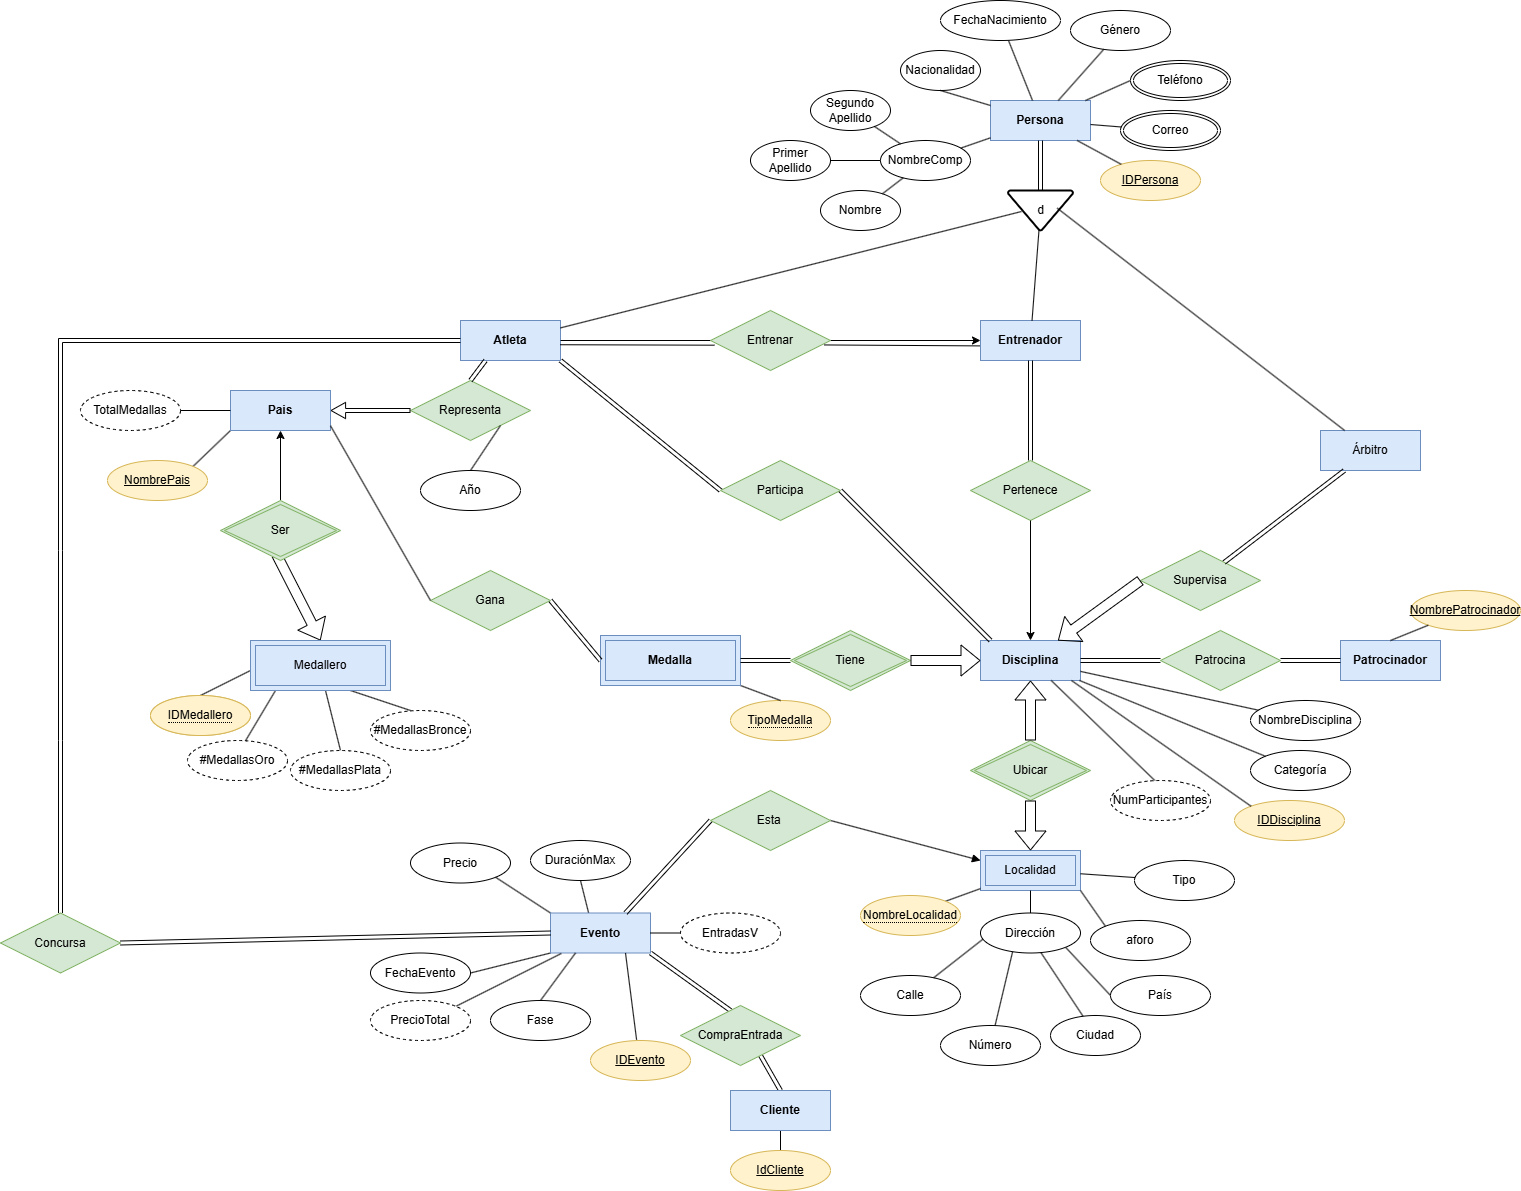
\includegraphics[width=1\textwidth]{resources/ModeloEntidad_Relación.png}

\end{figure}

\section{Modelo Relacional de la Práctica 4:}
\begin{figure}[H]
    \centering
    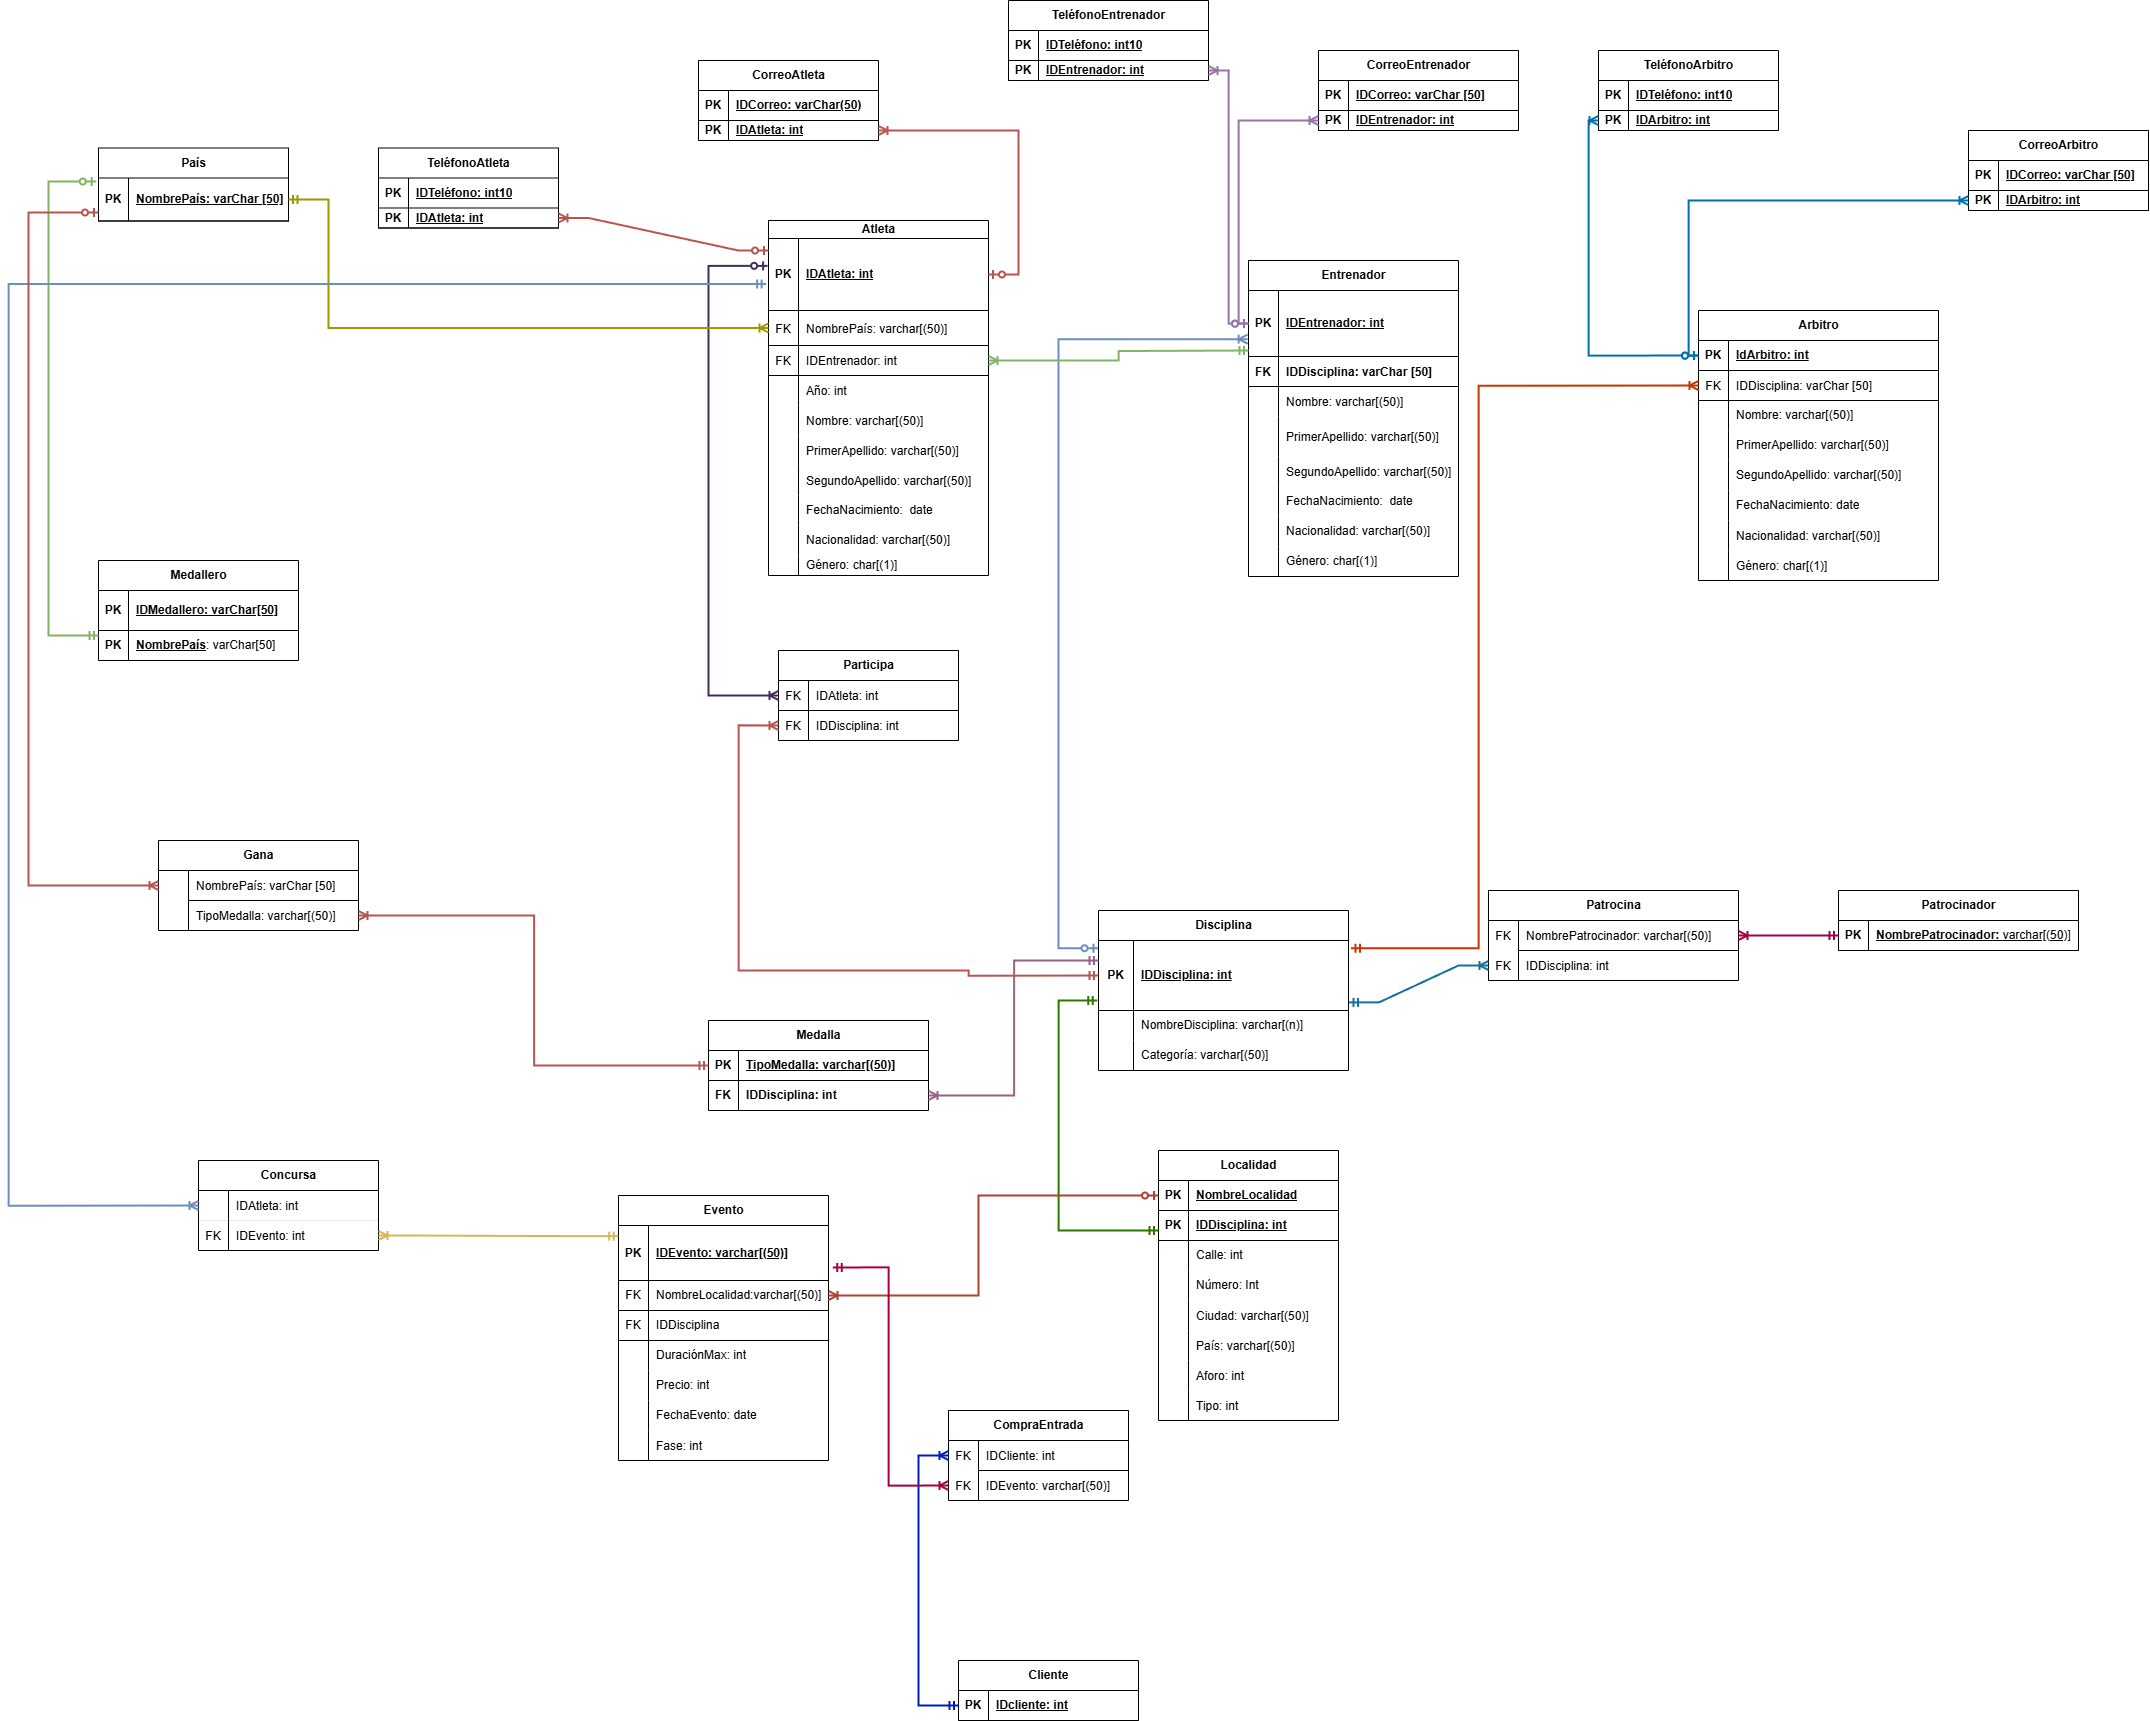
\includegraphics[width=1\textwidth]{resources/Modelo_Relacional.png}
\end{figure}


Y al final, ejecutando paso por paso el DDL.sql se obtiene la siguiente BDD relacional:
\section{Base de datos a partir del DDL.sql}
\begin{figure}[H]
    \centering
    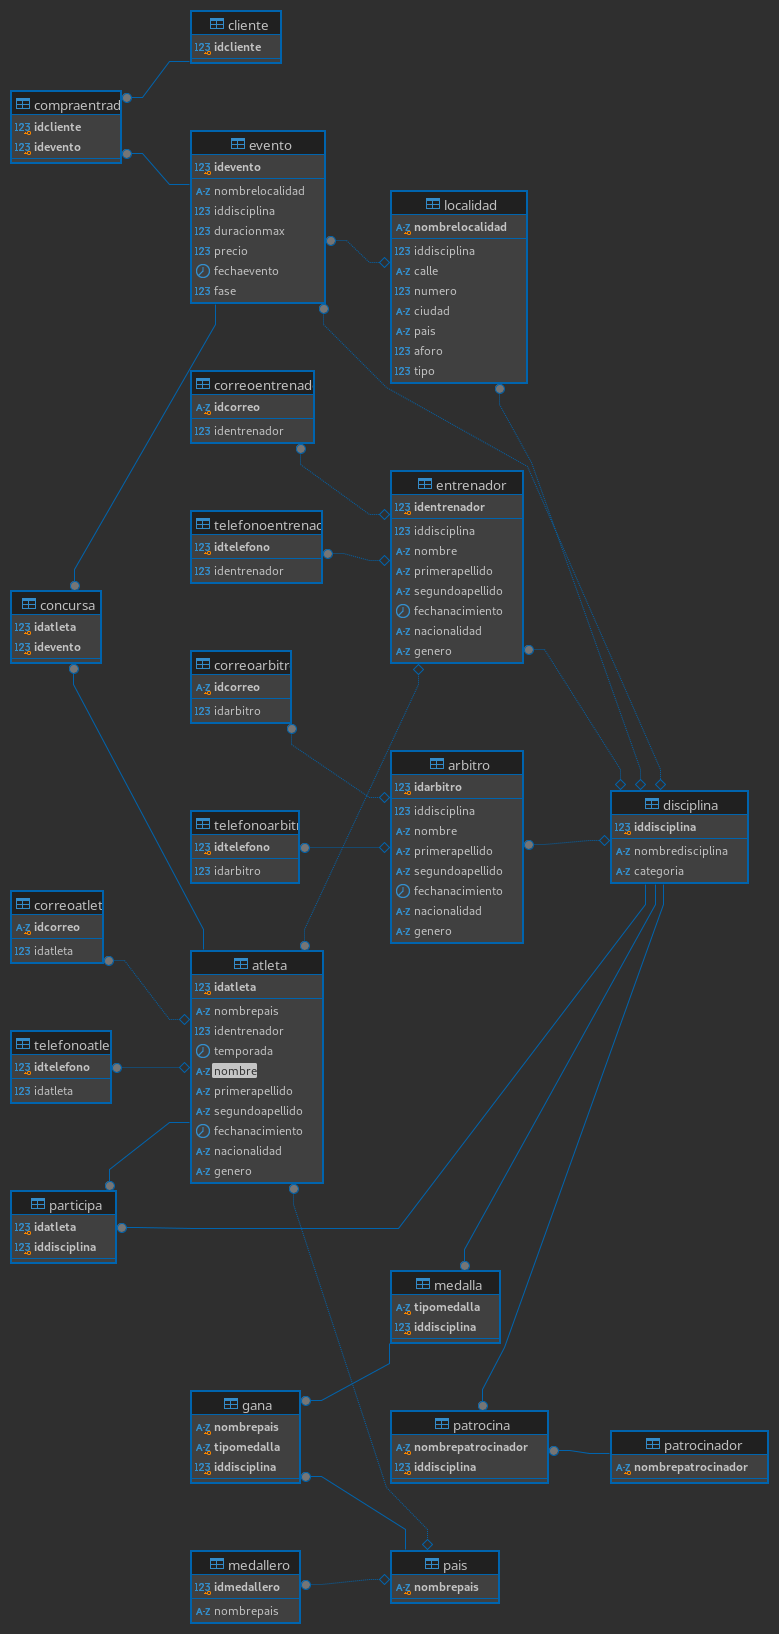
\includegraphics[height=.9\textwidth]{resources/bdd.png}
\end{figure}
        \end{enumerate}
    \newpage
    
\printbibliography
  
\end{document}